\begin{table}
  \caption{Notation used in this article}
  \centering
  \begin{tabular}{l l l}
    \hline
    \multicolumn{1}{c}{Type} &\multicolumn{1}{c}{Symbol} & \multicolumn{1}{c}{Quantity} \\
    \hline
    Genetic parameters & $\psi$ & \multicolumn{1}{p{10cm}}{Mgf of the mutational effect size distribution }\\
                             & $\frac{\theta}{2}$ & \multicolumn{1}{p{10cm}}{Per-locus mutation rate in units of coalescent time}\\
                             & $m_i$ &  \multicolumn{1}{p{10cm}}{$i^{th}$ non-central moment of the mutational effect size distribution}\\
                             & $\frac{\theta}{2}\mu_1$ & \multicolumn{1}{p{10cm}}{Rate of mutational bias in the infinitesimal limit}\\
                             & $\frac{\theta}{2}\mu_2$ & \multicolumn{1}{p{10cm}}{Rate of variance accumulation in the infinitesimal limit}\\
                             & $L$ & \multicolumn{1}{p{10cm}}{No. of potentially causal loci}\\
    Genealogies & $\mathbf{T}$ & \multicolumn{1}{p{10cm}}{Random vector of branch lengths representing the entire genealogy at a locus}\\
                             & $\Omega$ & \multicolumn{1}{p{10cm}}{Set of all possible branches for a given sample}\\
                             & $\omega$ & \multicolumn{1}{p{10cm}}{A particular branch in a genealogy defined by all individuals that branch subtends}\\
                             & $T_\omega$ & \multicolumn{1}{p{10cm}}{Length of branch $\omega$} \\
                             & $T_{MRCA}$ & \multicolumn{1}{p{10cm}}{Time to the most recent common ancestor at a particular locus}\\
                             & $\varphi_{\mathbf{T}}(\mathbf{s})$ & Mgf of the genealogy distribution \\
                             & $\mathbf{s}$ & Vector of dummy variables for each possible branch\\
                             & $s_\omega$ & Dummy variable for branch $\omega$ \\
                             & $\mathbbm{T}_{k,n}$ & \multicolumn{1}{p{10cm}}{For a sample of exchangeable lineages, the amount of time that $k$ lineages remain in a sample of size $n$}\\
                             & $\mathcal{T}_{i,j}$ & \multicolumn{1}{p{10cm}}{Pairwise coalescent time between a lineage in individual $i$ and a lineage in individual $j$}\\
                             & $\mathcal{T}_{A,B}$ & \multicolumn{1}{p{10cm}}{In a structured population, the pairwise coalescent time between a lineage sampled from population $A$ and a lineage sampled from population $B$}\\
                             & $\tau_{a+b}$ & \multicolumn{1}{p{10cm}}{Sum of all branches ancestral to both individuals $a$ and $b$}\\
                             & $\tau_{a/b}$ & \multicolumn{1}{p{10cm}}{Sum of all branches ancestral to individual $a$ but not $b$}\\
                             & $\Omega_{a+b}$ & \multicolumn{1}{p{10cm}}{Set of all branches ancestral to both individuals $a$ and $b$}\\
                             & $\Omega_{a/b}$ & \multicolumn{1}{p{10cm}}{Set of all branches ancestral to individual $a$ but not $b$}\\                           
    Trait values & $\mathbf{Y}$ & Random vector of trait values \\
                             & $Y_a$ & Trait value of individual $a$\\
                             & $\varphi_{\mathbf{Y}}(\mathbf{k})$ & Mgf of the trait value distribution \\
                             & $\mathbf{k}$ & \multicolumn{1}{p{10cm}}{Vector of dummy variables for each individual trait value}\\
                             & $k_a$ & Dummy variable for individual $a$\\
                             & $M_i$ & \multicolumn{1}{p{10cm}}{$i^{th}$ central moment of the trait value distribution in the entire population}\\
                             & $CVV$ & \multicolumn{1}{p{10cm}}{Coefficient of variation of trait variance over evolutionary realizations of a population}\\
                                       \hline
  \end{tabular}
\end{table}

In the model we investigate here, there are $L$ unlinked potentially causal loci
at which mutations influence the trait value. Following \citet{Kimura1969}, an
infinite number of mutations are possible within each locus and the rate per
unit of coalescent time at which mutations affecting the trait (causal
mutations) arise is $\T$. That is, $\T$ is the mutation rate for the entire
locus and not per nucleotide. An approximation for when at most one mutation per
locus is likely is considered in Section \ref{sec:lmr}. Mutations are randomly
assigned effects from a distribution of effect sizes, and effects are additive
both within and between loci. The moment generating function (mgf) of this
distribution is written as $\psi$ and the $i^{th}$ non-central moment is $m_i$.
Individuals are haploid and the sum of all mutations occurring in an
individual's history determines the trait value of the individual. An extension
to diploidly would be straightforward but is not considered here. Correlations
between individuals arise when mutations fall on shared portions of genealogies
at specific loci. Because the loci are unlinked we assume their genealogies are
independent. This model is shown schematically in Figure \ref{fig:schema}.

The genealogy at a locus is represented by the random vector of branch lengths,
$\mathbf{T}$. An element $T_{\omega}$ of $\mathbf{T}$ is the branch length
subtending only individuals in the set $\omega$ and no others in the sample. For
example, $T_{\{a,b\}}$ is the length of the branch subtending only individuals
$a$ and $b$. If a branch subtending only $a$ and $b$ does not exist for a given
genealogy, $T_{\{a,b\}}$ is set to zero. In this way $\mathbf{T}$ encodes both
the branch lengths and the topology of a genealogy. $\Omega$ is the set of all
possible branches. If there are three sampled individuals, $a$, $b$, and $c$,
then $\Omega=\{\{a\},\{b\},\{c\},\{a,b\},\{a,c\},\{b,c\}\}$ and
$\mathbf{T}=(T_{\{a\}},T_{\{b\}},T_{\{c\}},T_{\{a,b\}},T_{\{a,c\}},T_{\{b,c\}})$.
The mgf for the distribution of branch lengths is denoted $\varphi_{\mathbf{T}}$.

Phenotypic trait values are the random quantities we are interested in and
result from mutations occuring along the branches of genealogies. We will
hereafter refer to the phenotypic trait simply as trait values and ignore any
environmental component. The random vector of trait values in the sampled
individuals is $\mathbf{Y}$. If we had sampled individuals $a$, $b$, and $c$,
then $\mathbf{Y}=(Y_a,Y_b,Y_c)$. The contribution to the trait values from a
single locus is the change relative to the value in the most recent common
ancestor (MRCA) of the sample at that locus. Since we do not know the ancestral
value, we cannot directly observe the change in trait values. Thus, for a trait
controlled by multiple loci, $\mathbf{Y}$ is the sum over contributions from
these loci, each measured with respect to an arbitrary value. However,
$\mathbf{Y}$ is sufficient to determine measurable quantities such as
differences in trait values between individuals as well as the sample variance.
The moment generating functions for the distribution of trait values is denoted
$\varphi_{\mathbf{Y}}$.

\begin{figure}
  \centering
  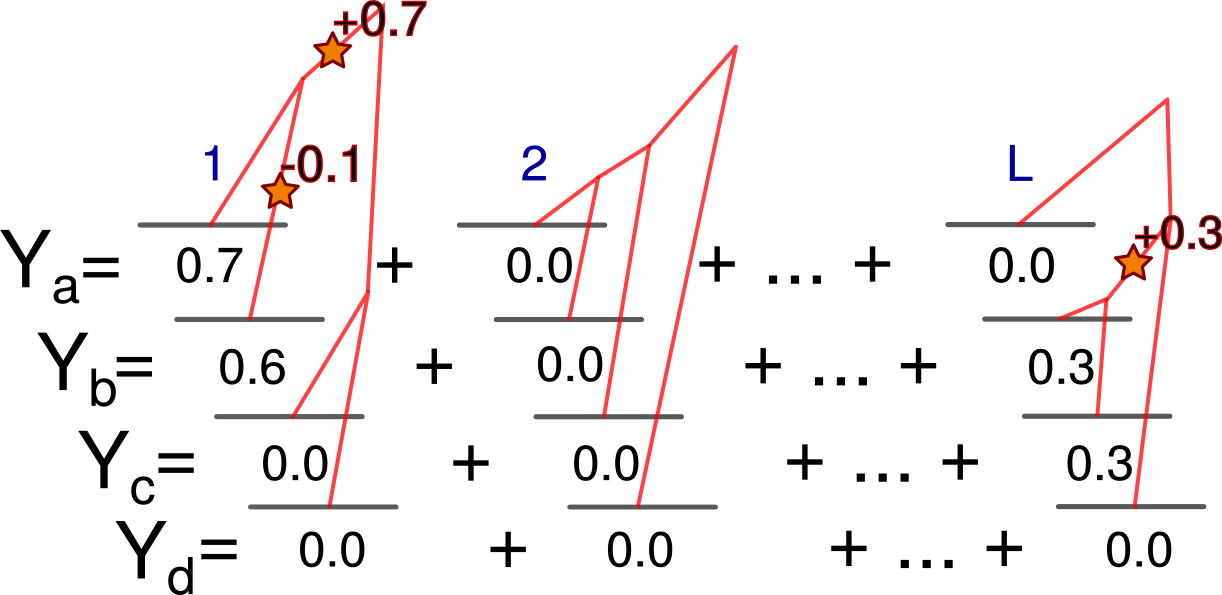
\includegraphics[width=0.9\textwidth]{./figures/schema.png}

  \caption{\textbf{A schematic representation of the model for how trait
  distributions arise from genealogical and mutational processes.} $L$ loci
  potentially affect the trait in a set of individuals and have independent
  genealogies. Mutations occur within loci as a Poisson process and act
  additively to give individual trait values. Many loci with the potential to
  affect the trait may receive no mutations.}

  \label{fig:schema}
\end{figure}

Here we refer to the genetic parameters of a trait as the combination of
quantities not influenced by the genealogical process: ($L$, $\T$, $\psi$).
Another quantity useful for describing a trait's distribution is its sparsity.
Sparsity should reflect how many mutations segregating in the population
influence the trait, with a more `sparse' trait being one affected by fewer
segregating mutations. Formally, we measure sparsity as the average number of
pairwise differences between two randomly chosen haplotypes at loci affecting
the trait. A trait with fewer causal pairwise differences is more sparse.
Sparsity thus depends both on the genetic parameters through the mutation rate,
the number of potentially causal loci, and the distribution of coalescence
times.

In populations of exchangeable individuals, a useful way to summarize the
distribution of genealogies is through the moments of $\mathbbm{T}_{k,n}$ which
denotes the amount of time that $k$ lineages remain in the genealogy of a sample
of size $n$. The pairwise coalescent time between a lineage in individual $i$
and in individual $j$ is written as $\mathcal{T}_{i,j}$. When considering
structured populations, $\mathcal{T}_{a,b}$ is also used to denote the
coalescence time between a randomly chosen lineage from subpopulation $a$ and a
randomly chosen lineage from subpopulation $b$. A final set of quantities are
defined for sums of branch lengths. Let $\tau_{a+b}$ be the sum of all branches
ancestral to both $a$ and $b$, and $\tau_{a/b}$ be the sum of all branches
ancestral to $a$ but not $b$. Extensions of this for more than two individuals
are also used. The same notation is used when referring to sets of branch
indices. So $\Omega_{a+b}$ and $\Omega_{a/b}$ would be the sets of branches
added to get $\tau_{a+b}$ and $\tau_{a/b}$ respectively.

%%% Local Variables:
%%% TeX-master: "short_report.tex"
%%% End:
